% !TEX root = ../notes_template.tex
\chapter*{머리말}
\addcontentsline{toc}{chapter}{머리말}
\minitoc

우선 복소함수론은 무엇이고 왜 중요한지 간단히 살펴보자.
복소수라는 개념 만큼은 다들 언젠가 배웠을 것이므로 
복소수에 친숙하다는 가정하에 이야기를 전개한다.
1장과 그 이후에 개념을 처음부터 만들어갈 예정이니
독자들은 머리말에서 이해하지 못한 부분에 대하여 걱정할 필요는 없다.

%=====
\section*{복소해석학이란?}
실해석학(real analysis)에서는 실수에 대한 미적분을 엄밀하게 정의하며
실수열의 수렴성, 실변수 함수의 연속성, 미분, 적분의 개념을 공부한다.
이를 바탕으로 복소해석학(complex analysis)은
복소수를 대상으로 하여 유사한 개념들을 공부하는 것으로 추측해 볼 수 있다.
이 예상은 부분적으로 참이다.
미분을 공부하기 전까지는 실해석학과 비교할 때 복소해석학만의
새로운 특징이 보이지 않는다.
하지만 미분부터는 복소해석학과 실해석학의 근본적인 차이가 나타난다.
따라서 복소해석학은 해석학을 복소수 범위로 단순 확장한 것이 아니며, 훨씬 더 특별한 의미를 갖는다.

%\begin{center}
\fbox{\begin{minipage}{\dimexpr\textwidth-15\fboxsep-2\fboxrule\relax}
\begin{center}
복소해석학은 ``{\bf 복소 의미로 미분가능한}'' 함수를 다룬다.
\end{center}
\end{minipage}}
%\end{center}

실변수 함수 $f:\mathbb R \to \mathbb R$에 대하여
$$
\lim_{x\to x_0} \frac{f(x)-f(x_0)}{x-x_0} = L
$$
을 만족하는 실수 $L$이 존재하면 
함수 $f$가 $x_0\in \mathbb R$에서 {\bf 미분가능}하다고 한다.
즉, 모든 $\epsilon>0\,$에 대하여,  대응되는 $\delta>0\,$가 존재하여
$$
0<|x-x_0|<\delta \text{ 이면 }
\left| \frac{f(x)-f(x_0)}{x-x_0} - L\right| < \epsilon \text{ 을 만족한다.}
$$
다른 방법으로 표현하면, 
거리 $\epsilon$이 주어질 때,
$x_0$는 아니면서 충분히 가까운 모든 $x$에 대하여 변화율
$$
 \frac{f(x)-f(x_0)}{x-x_0}
$$
와 실수 $L$의 거리가 $\epsilon$보다 작게 만들 수 있다.

같은 방법으로, 복소함수 $f:\mathbb C \to \mathbb C$에 대하여
$$
\lim_{z\to z_0} \frac{f(z)-f(z_0)}{z-z_0} = L
$$
을 만족하는 복소수 $L$이 존재하면 
복소함수 $f$가 
$z_0\in \mathbb C$에서 {\bf 복소미분가능}하다고 한다.
즉, 모든 $\epsilon>0\,$에 대하여, 대응되는 $\delta>0\,$가  존재하여
$$
0<|z-z_0|<\delta \text{ 이면 }
\left| \frac{f(z)-f(z_0)}{z-z_0} - L\right| < \epsilon \text{ 을 만족한다.}
$$

유일한 차이는 {\bf 복소수 절대값}으로 거리를 나타낸 것 뿐이며
직관적인 방법으로 
실변수 함수의 미분을 일반화 한 것으로 보인다.

하지만, 단순한 일반화로 생각했던 것과는 달리 깊은 차이가 있으며,
복소미분 가능한 함수들의 집합은  미분가능한 실변수 함수들의 집합과는 근본적인 차이가 있음을 살펴볼 것이다.
이와 관련된 예제를 살펴보자.

\begin{salt_example}
함수 $f:\mathbb R \to \mathbb R$를
$ f(x) = \begin{cases} x^2, & x\ge 0, \\ -x^2, & x<0 \end{cases}$
라고 정의하자.

\begin{figure}[!h]
\begin{center}
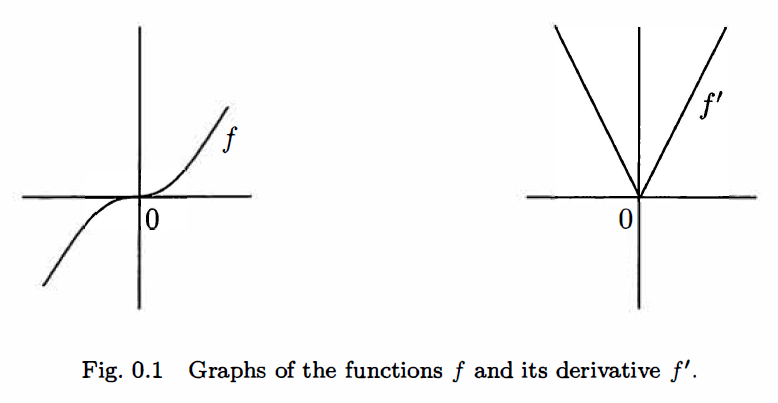
\includegraphics[width=0.6\textwidth]{./SaltChapter/preface-fig-0-1}
\end{center}
\label{fig:0.1}
\caption{함수 $f$와 도함수 $f'$의 그래프}
\end{figure}

그러면 $f$는 모든 점에서 미분가능하며 다음과 같이 쓸 수 있다.
\begin{equation}\label{eq0.1}
f'(x) = \begin{cases} 2x, & x\ge 0, \\ -2x, & x<0. \end{cases}
\end{equation}
$x\ne0$일 때는 $f'(x)$를 직접 계산하여 구할 수 있고,
$f'(0)=0$임을 다음과 같이 보일 수 있다. \\
$x\ne0$에 대하여
$$
\left| \frac{f(x) - f(0)}{x-0} - 0\right|  = \left| \frac{f(x)}{x}\right| = \frac{|x|^2}{|x|} = |x| = |x-0|
$$
이므로 주어진 $\epsilon>0\,$에 대하여 
$\delta = \epsilon (>0)$으로 잡으면
$0<|x-0|<\delta$일 때, 
$$
\left| \frac{f(x) - f(0)}{x-0} - 0\right|  = |x-0| <\delta = \epsilon
$$
을 얻는다.
하지만, $f'$은 원점 $x=0$에서 미분가능하지 않다.
증명은 연습문제 \ref{ex-0-1}를 참고하라.
요약하면, 함수 $f:\mathbb R \to \mathbb R$는 모든 실수에서 미분가능하지만 
그 도함수 $f'$은 모든 점에서 미분이 가능하지는 않다.

이와 대조적으로, 복소함수 $F:\mathbb C \to \mathbb C$가
모든 복소수에서 복소미분가능하다면, 무한번 복소미분가능함을 공부할 예정이다.
특히, 도함수 $F'$도 모든 복소수에서 복소미분가능하다.
실해석학에 익숙하다면 이는 분명 예상을 벗어난 결과이다.
우리는 복소해석학에서 이러한 놀라운 결과가 발생하는 이유에 대하여 살펴볼 예정인데,
복소미분가능하다는 것은 이러한 현상을 가능하게 하는 ``엄밀한'' 조건을 내포하고 있다.
또한, 이 엄밀함은 복소수의 곱셈의 기하학적인 특성에 따른 결과임을 보일 것이다.
\hfill $\diamondsuit$
\end{salt_example}

\begin{salt_exercise} \label{ex-0-1}
식 \eqref{eq0.1}에서 정의된 함수 $f':\mathbb R \to \mathbb R$는 $0$에서 미분 불가능함을 보여라.
\end{salt_exercise}

%=====
\section*{왜 복소해석학을 공부하는가?}

복소해석학이 단지 실해석학의 색다른 일반화로만 보일지 모르지만 사실 그렇지 않다. 
복소해석학은 수학의 모든 분야에서 필수적이다.
실제로 실해석학과 복소해석학은 뗄 수 없는 관계에 있으며,
응용 과학분야에서도 복소해석학은 중요한 역할을 하고 있음을 살펴볼 예정이다.
여기서는 복소해석학을 공부해야 하는 몇가지 이유를 간단히 나열해보자.

\begin{itemize}
\item[(1)] {\bf 편미분방정식:}  복소미분가능한 함수 $f:\mathbb C \to \mathbb C$ 의 
실수부와 허수부 $u,v: \mathbb R^2 \to \mathbb R\,$는 실함수가 되며, 
$(x,y)\in \mathbb R^2$에 대하여 $u(x,y) := \Re(f(x,y))$, $v(x,y):=\Im(f(x,y))$로 쓸 수 있다.

\begin{figure}[!h]
\begin{center}
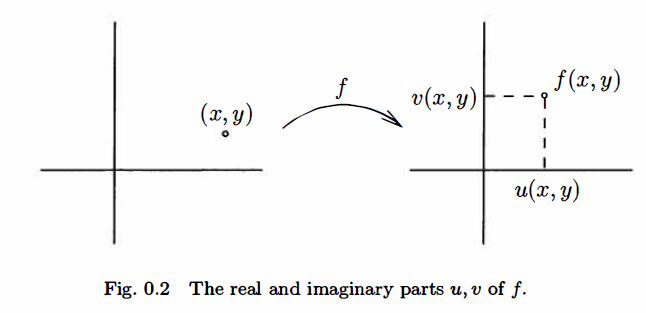
\includegraphics[width=0.5\textwidth]{./SaltChapter/preface-fig-0-2}
\end{center}
\label{fig:0.2}
\caption{복소함수 $f$의 실수부 $u$와 허수부 $v$}
\end{figure}

실수부와 허수부는 라플라스 방정식이라 불리는 중요한 편미분방정식을 만족한다:
$$
\Delta u := \frac{\partial^2 u}{\partial x^2} + \frac{\partial^2 u}{\partial y^2} = 0.
$$
마찬가지로 $\Delta v=0$도 성립한다.
라플라스 방정식은 물리학과 같은 많은 응용문제에서 유도되는 중요한 방정식이다.
예를 들면, 전자기학, 시간에 불변하는 열전도 방정식, 비압축성 유체, 브라운 운동 등에 사용된다.

\item[(2)] {\bf 실해석:} 복소해석학을 이용하면, 다음 실적분을  쉽게 계산할 수 있다.
$$
\int_{-\infty}^\infty \frac{\cos x}{1+x^2}dx, 
\quad
\int_0^\infty \cos(x^2)dx.
$$
이 문제들은 실수에서 정의된 것이나 복소해석학을 이용하여 풀 수 있다.

또한, 복소해석학을 이용하면 실해석학에서 발생하는 문제들을 명확히 할 수 있다.
예를 들어 다음 함수를 생각해보자.
$$
f(x):= \frac{1}{1-x^2}, \quad
x\in \mathbb R \setminus \{-1,1\}.
$$
그러면 $f$는 $x=\pm1$에서 정의되지 않아 특이점을 갖는다.
하지만, 구간 $(-1,1)$에서는 잘 정의된다.
등비급수
$$
1+x^2+x^4+x^6 +\cdots
$$
는  $|x^2|<1$에서, 즉, $|x|<1$에서 수렴하므로 $x\in (-1,1)$에 대하여
$$
1+x^2+x^4+x^6 +\cdots = \frac{1}{1-x^2} = f(x).
$$
$f$가 $x=1$과 $x=-1$에서 특이점을 가지므로 위의 급수표현은 $x\in(-1,1)$에 대해서만 유효함은 당연해 보인다.
이제 새로운 함수 $g$를 다음과 같이 생각해보자.
$$
g(x):= \frac1{1+x^2}, \quad x\in \mathbb R.
$$
등비급수
$$
1-x^2+x^4-x^6 +\cdots
$$
는  $|-x^2|<1$에서, 즉, $|x|<1$에서 수렴하므로 $x\in (-1,1)$에 대하여
$$
1-x^2+x^4-x^6 +\cdots = \frac{1}{1+x^2} = g(x).
$$
따라서 
$g$는 $x=1$과 $x=-1$에서 특별히 문제가 될 이유가 없음에도 불구하고
함수 $g$도 $x\in(-1,1)$에 대해서만 유효한 급수표현을 갖는다.
이 미스테리는 책의 후반부에서 해결할 예정이며 다음 복소함수를 살펴볼 필요가 있다.
$$
F(z) = \frac1{1-z^2} \quad
G(z) = \frac1{1+z^2}
$$
두 함수의 정의역을 $\mathbb R$로 한정하면 각각 $f$와 $g$를 얻는다.
특히, 복소함수 $G$는 이제 $z=\pm i$에서 특이점을 갖는다.
그림에서 $z=0$을 중심으로 급수 전개가 유효한 최대 원판은
$G$의 특이점을 포함하지 않아야 함을 알 수 있다.

\begin{figure}[!h]
\begin{center}
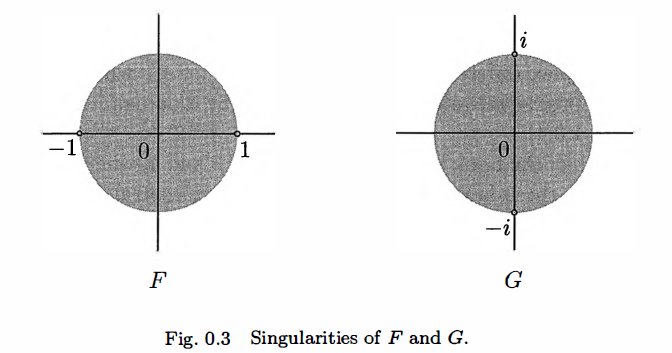
\includegraphics[width=0.6\textwidth]{./SaltChapter/preface-fig-0-3}
\end{center}
\label{fig:0.3}
\caption{복소함수 $F$와 $G$의 특이점}
\end{figure}

\item[(3)] {\bf 응용 문제:}  푸리에 변환, 라플라스 변환, z-변환과 같이 응용 문제 해결에 사용되는 많은 도구들은
복소함수 이론에 의존한다. 이  도구들은 여러 응용 분야에서 나타나는 미분방정식의 해결에 유용하다.
복소해석학은 수리물리와 공학분야의 응용에 중요한데, 예를 들면, 제어이론, 신호처리 등이 있다.

\item[(4)] {\bf 해석 정수론:}
자연수와 관련된 많은 문제가 복소해석학을 이용하여 해결된다는 것은 아마도 놀라울 것이다.
예를 들면, 소수정리는 큰 자연수 $n$에 대하여 $n$보다 작은 소수의 개수 $\pi(n)$을 
점근적으로 판정하는 방법을 알려준다.

\begin{salt_theorem}{\bf (소수정리)}
$$
\lim_{n\to\infty} \frac{\pi(n)}{n/(\log n)} = 1.
$$
\end{salt_theorem}

소수정리는 리만 제타함수라는 복소미분가능 함수의 성질을 이용하여 증명할 수 있음이 밝혀졌다.
리만 제타함수와 관련된 해석 정수론의 유명한 미해결 문제로 리만가설이 있다.
리만 제타함수의 모든 비자명해는 복소평면에서 직선 $\Re(s)=\frac12$ 위에 존재한다는 것이다.
우리는 리만 제타함수를 연습문제 \ref{ex-4-5}에서 만날 것이다.
\end{itemize}


\section*{복소해석학에서는 무엇을 배우는가?'}

이 과정의 중심이 되는 주제는 다음과 같다.

%\begin{center}
\fbox{\begin{minipage}{\dimexpr\textwidth-15\fboxsep-2\fboxrule\relax}
\begin{center}
복소영역에 정의된 복소해석함수들
\end{center}
\end{minipage}}
%\end{center}

즉, 복소영역 $D$에 정의된 복소미분가능 함수 $f \colon D\to \mathbb C$가 대상이다.
``복소영역'' $D$에 대한 정확한 의미는 1.3.4 절에서 다룬다.

책의 중심인 2, 3, 4장에서는 
핵심 주제인 복소해석(holomorphic) 함수에 빛을 비춰줄 다음 3가지를 다룬다.
\begin{enumerate}
\item[(1)] 코시-리만 방정식
\item[(2)] 코시 적분 정리
\item[(3)] 테일러 급수
\end{enumerate}

\begin{figure}[!h]
\begin{center}
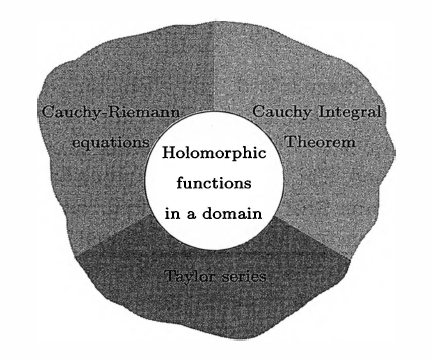
\includegraphics[width=0.5\textwidth]{./SaltChapter/preface-fig-0-4}
\end{center}
\end{figure}

%다음 정리는 책에서 공부할 핵심적인 내용을 요약한 것이다.
다음은 이 책의 핵심정리이다.

\begin{salt_theorem}
경로연결된 열린집합 $D$에 정의된 함수
$f:D\to \mathbb C$에 대하여 다음은 동치이다.
\begin{itemize}
\item[(1)] $D$의 모든 점 $z$에서 $f'(z)$가 존재한다.
\item[(2)] $D$의 모든 점 $z$에서 모든 차수 ($n\ge0$)의 미분  $f^{(n)}(z)$가 존재한다.
\item[(3)] 실수부와 허수부 $u:=\Re(f)$, $v:=\Im(f)$는 연속미분가능하며 
$$
\frac{\partial u}{\partial x} = \frac{\partial v}{\partial y},
\quad
\frac{\partial u}{\partial y} = - \frac{\partial v}{\partial x}
$$
을 만족한다.
\item[(4)] $D$의 단순연결 부분영역 $S$에 대하여 
복소해석함수 $ F: S\to \mathbb C$가 존재하여
$S$의 모든 점 $z$에서 $F'(z)= f(z)$를 만족한다.
\item[(5)] $ f$ 가 $D$에서 연속이고, 
$D$의 모든 단순연결 부분영역에서
임의의 조각마다 매끄러운 닫힌곡선 $\gamma$에 대하여 다음이 조건이 성립한다.
$$
\int_\gamma f(z)dz = 0.
$$
\item[(6)] $\{ z\in \mathbb C\,:\, |z-z_0| \le r \} \subset D$이면
$|z-z_0|<r$을 만족하는 임의의 $z$에 대하여
$$
f(z) = \sum_{n=0}^\infty c_n(z-z_0)^n
$$
을 만족하는 복소수열 $(c_n)_{n\ge0}$이 유일하게 존재한다.
부가적으로 계수 $c_n$는 다음식으로 구할 수 있다.
$$
c_n = \dfrac1{2\pi i} \dint_{|\zeta-z_0|=r} \frac{f(\zeta)}{(\zeta-z_0)^{n+1}}d\zeta = \dfrac{f^{(n)}(z_0)}{n!}.
$$
\end{itemize}
\end{salt_theorem}

\section*{복소해석학은 복잡한 해석학이 아니다!}


실제로 아주 복잡한 것이 아니며,  지나치게 해석적인 것도 아니다.
복소해석학은 실해석학보나 오히려 유연하다.
복소미분의 핵심 개념 몇가지를 정립하고 나면 
입실론-델타($\epsilon$-$\delta$)를 포함한 정교한 기법들은 적게 사용된다.
앞의 핵심정리를 보면 실해석학과 근본적으로 다른 결과가 도출됨을 예상할 수 있다.
예를 들어 실함수가 열린구간 $(a,b)$에 정의된 미분가능할 때 그 도함수는 연속함수가 아닐 수 있다.
반면 복소평면 $\mathbb C$의 열린집합에 정의된 복소미분가능함수는 
무한번 미분가능하다!
그 이유는 복소곱셈이 특별한 기하학적 의미를 갖기 때문인데
복소미분가능함수는 국소적인 성질로 전체가 규정되며 
함수값을 임의로 매핑하는 것을 허용하지 않는다.
이렇게 제어되는 성질이 복소함수를 한정적으로 만드는데
2.3절에서 이를 자세히 살펴볼 예정이다.
그럼에도 불구하고 자명하지 않으며 충분히 흥미로운 주제이다!

\section*{대상 독자}

복소함수론은 미적분학과 다변수 미적분학을 학습한 학생을 대상으로 하는 기초 과정이다.
책의 제목에서 짐작할 수 있듯이
가장 최소한의 선수지식으로 학습할 수 있는 복소함수의 핵심적인 내용을 담고 있다.
이 책은 저자가 수학과 및 경제학과 3학년 학생을 대상으로 강의했던 강의록을 
바탕으로  만들어졌다.


\section*{감사의 글}

 많은 유용한 의견을 보내준 
Raymond Mortini, Adam Ostazewski, Rudolf Rupp에게 감사드린다.
참고문헌 목록에 있는 기존 학습자료에 의존하였으며
이는 연습문제의 경우도 마찬가지다.
몇가지 경우는 각 장의 끝에 ``참고'' 절을 넣고 상세한 참고문헌을 제시했지만
참고 절을 넣지 않은 경우에도 이 책만의 독창성을 주장하는 것은 아니다.

\begin{flushright}
2013년, 런던과 룬트에서

Sara Maad Sasane과 Amol Sasane
\end{flushright}

